\documentclass[11pt]{extarticle}
\usepackage{amssymb}
\usepackage{epsfig}

\setlength{\oddsidemargin}{0.25 in}
\setlength{\evensidemargin}{-0.25 in}
\setlength{\topmargin}{-0.6 in}
\setlength{\textwidth}{6.5 in}
\setlength{\textheight}{8.5 in}
\setlength{\headsep}{0.75 in}
\setlength{\parindent}{0 in}
\setlength{\parskip}{0.1 in}

\newenvironment{Section}[2]{
  \section*{\huge{Section #1:\\ #2}}
}

\newcommand{\itab}[1]{\hspace{0em}\rlap{#1}}
\newcommand{\tab}[1]{\hspace{.2\textwidth}\rlap{#1}}

\newcommand{\lecture}[4]{
   \pagestyle{myheadings}
   \thispagestyle{plain}
   \newpage
   \setcounter{page}{1}
   \noindent
   \begin{center}
   \framebox{
      \vbox{\vspace{2mm}
    \hbox to 6.28in { {\bf 20CS6037 Machine Learning \hfill} }
       \vspace{6mm}
       \hbox to 6.28in { {\Large \hfill #1 (#2)  \hfill} }
       \vspace{6mm}
       \hbox to 6.28in { {\it Lecturer: #3 \hfill Scribes: #4} }
      \vspace{2mm}}
   }
   \end{center}
   \markboth{#1}{#1}
   \vspace*{4mm}
}

%Send your finished notes to the instructor
%({\tt ancaralescu@gmail.com}), including the Latex file and all .eps
%or .pdf files that you've created for figures. Double-check that your file compiles with {\tt pdflatex lec1.tex} before you send it.

%These notes should be complete, correct, clear, and free of typos.

\begin{document}

\lecture{MLE, MAP, Bayesian Reasoning - Chapter 3 \& 5} {Lecture 5: 9/9/14}{Anca Ralescu}{Khaldoon Ashouiliy, Kyungmook Park}

\begin{Section}{1}{Conditional Independence}
\end{Section}
\begin{Section}{2}{Transformation of Random Variables}
\end{Section}
\begin{Section}{3}{General Transformations}
\end{Section}
\begin{Section}{4}{Monte Carlo Approximation}
\end{Section}
\begin{Section}{5}{Entropy}
\end{Section}
\begin{Section}{6}{Mutual Information}
\end{Section}



\newpage

\begin{Section}{1}{Conditional Independence}
\Large{X,Y r.v. X $\perp Y$ : X and Y are independent\\\\
\underline{Def}\\
X $\perp$ Y $\Leftrightarrow$ P(X,Y) = P(X)P(Y)\\
This really means \{w $\in$ S $|$ X(w) = a\}, \{w $\in$ S $|$ Y(w) = b\}\\
are independent event for all a $\in$ Range(x); b $\in$ Range(Y)

\underline{Notation}\\
X $\perp$ Y $|$ 2 : X and Y are \textbf{\textit{Conditionally Independent} (CI)} given 2\\

P(X $\perp$ Y $|$ 2) $\Leftrightarrow$ P(X, Y $|$ 2) = P(X $|$ 2)P(Y $|$ 2)\\

\begin{figure}[htbp] %  figure placement: here, top, bottom, or page
   \centering
			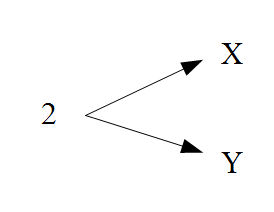
\includegraphics[width=2in]{Figure1.png}
  % \includegraphics[width=2in]{name.pdf} % uncomment this line and put the figure in the same folder as this document.
   \caption{X and Y are CI given 2}
   \label{fig:Figure1}
\end{figure}

\underline{P}(X, Y) : Joint Distribution of X and Y\\
\{w $\in$ S $|$ X(w) = a\}, \{w $\in$ S $|$ Y(w) = b\}\\
Can extend to \underline{P}(X$_1$, $\ldots$ , X$_D$) : CDF, PDF/PMF\\
\itab{COV(X, Y)} \tab{$\triangleq$ E[(X-E(X))(Y-E(Y))]}\\
\itab{}\tab{ = E[XY - XE(Y) - YE(X) + E(X)E(Y)]}\\
\itab{}\tab{ = E(XY) = E(X)E(Y)}\\

\newpage

For a vector X = (X$_1$, X$_2$, X$_3$)\\

\[
Cov [X] =
\left[ {\begin{array}{ccc}
Var(X_1) & Cov(X_1,X_2) & Cov(X_1,X_3) \\
Cov(X_2,X_1) & Var(X_2) & Cov(X_2,X_3) \\
Cov(X_3,X_1) & Cov(X_3,X_2) & Var(X_3) \\
\end{array} } \right]
\]

Cov $\in$ (0, $\infty$)\\

\underline{Correlation} $P$(X,Y) = $\frac{Cov(X,Y)}{\sqrt{Var(X)Var(Y)}}$ $\in$ [-1,1]\\

X, Y independent $\Rightarrow$ Cov(X,Y) = 0 $\Rightarrow$ $P$(X,Y) = 0 (Uncorrelated)\\

Independence $\rightleftharpoons$ Uncorrelated\\

ex)\\
X $\sim$ u(-1,1) ; Y = X$^2$ $\Rightarrow$ X, Y are dependent\\
$P$(X,Y) = 0\\

E(X) = $\frac{-1+1}{2}$ = 0  Var(X) = $\frac{(1-(-1)^2}{12}$ = $\frac{4}{12}$ = $\frac{1}{3}$\\\\\\
\itab{E(Y)}\tab{= $\int_{-1}^1x^2f(x)dx$}\\
\itab{}\tab{= $\int_{-1}^1x^2(\frac{1}{2})dx$=$\frac{1}{2}\frac{x^4}{4}\arrowvert_{-1}^1 = \frac{2}{6} = \frac{1}{3}$}\\

E(XY) = $\int_{-1}^1x^3\frac{1}{2}dx = \frac{1}{2}\frac{x^4}{4}\arrowvert_{-1}^1 = \frac{1}{2}\cdot0$\\

Cov(X,Y) = E(XY) - E(X)E(Y) = 0 - 0 $\cdot$ $\frac{1}{3}$ = 0 - 0 = 0\\

} %End of \Large
\end{Section}

\newpage

\begin{Section}{2}{Transformation of Random Variables}

\Large{

X $\sim$ P(X)   p:pdf\\
Y = f(X)    What is the distribution of Y?\\
$P_Y(Y \leq y) = P_Y(f(X) \leq y) = \underline{P}_X(X \leq f^{-1}(y)) = P(f^{-1}(y))$\\

ex) Y = aX+b $\Rightarrow$ f(x) = aX+b\\

\itab{f$^{-1}$(y) = $\frac{y-b}{a}$}\tab{X = -1 Y = b-a ; X = 1 Y = a+b}\\

P$_Y$(y) = P$_X$ ($\frac{y-b}{a}$)\\

ex) X $\sim$ u(-1,1)

\begin{figure}[htbp] %  figure placement: here, top, bottom, or page
   \centering
			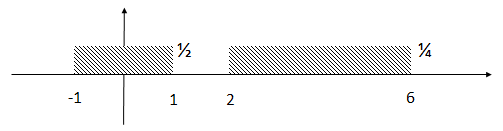
\includegraphics[width=6in]{Figure2.png}
  % \includegraphics[width=2in]{name.pdf} % uncomment this line and put the figure in the same folder as this document.
   \caption{Result of Transformation}
   \label{fig:Figure2}
\end{figure}

\[
P_X(x) =
\left\{ {\begin{array}{cc}
0 & x \leq -1 \\
\frac{1}{2} & -1 < X < 1 \\
0 & x \geq 1 \\
\end{array} } \right.
\]

\[
P_X(\frac{y-b}{a}) =
\left\{ {\begin{array}{cc}
0 & \frac{y-b}{a} \leq -1 \\
\frac{1}{b-a+a+b} & -1 < \frac{y-b}{a} < 1 \\
0 & x \geq 1 \\
\end{array} } \right.
= \left\{ {\begin{array}{cc}
0 & \frac{y-b}{a} \leq -1 \\
\frac{1}{4} & -1 < \frac{y-b}{a} < 1 \\
0 & x \geq 1 \\
\end{array} } \right.
\]

\[
\left\{ {\begin{array}{cc}
E(y) = &a E(x) + b \\
Var(y) = &a^2 E(x) \\
\end{array} } \right.
\]

For multivariable case : X = ($X_1$, \ldots, X$_n$), y=a$^T$x+b\\
E(y) = y=a$^T$E(x)+b\\

} %End of \Large

\end{Section}
\begin{Section}{3}{General Transformations}
\Large{
\underline{Discrete Case} X $\sim$ u(1, \ldots, 4)\\
P(x=i) = $\frac{1}{4}$ i=1,2,3,4\\
\[
Y=
\left\{ {\begin{array}{cc}
1& if\;X\;is\;even \\
0& if\;X\;is\;odd \\
\end{array} } \right.
\]

\itab{\underline{P}(y = 1)}\tab{= $P_x$ (x is even)}\\
\itab{}\tab{$\sum{P_x(X=k)\;=\;P(X=2)+P(X=4)=\frac{2}{4}=\frac{1}{2}}$}\\

k $\in$ \{1, 2, 3, 4\}\\
k is even\\

P(y=0) = \ldots = $\frac{1}{2}$\\

\underline{Continuous Case}\\
\itab{X $\sim$ $P_x$)(x)}\tab{:pdf}\\
\itab{Y = f(X)}\tab{$\Rightarrow$ $P_Y$(y) = ?}\\

Use cdf
$P_Y$(Y$\leq$y) = $P_Y$(f(X)$\leq$y) = $P_X$(X$\leq$f$^{-1}$(y)) = $P_X$(f$^{-1}$(y))\\

Provided that f is invertible\\
Then $P_Y$(y) the pdf of Y is obtained by taking the derivative of cdf of Y\\

$P_Y$(y)=$\frac{d}{dy}P_Y$(Y$\leq$y)=$\frac{d}{dy}P_X$(f$^{-1}$(y))=$\frac{d}{dx}P_X$(x)$\cdot\frac{dx}{dy}$\\
\itab{Where x=f$^{-1}$(y)}\tab{  $\;\;\;$ignore sign of $\frac{dx}{dy}$}\\
$\Rightarrow P_Y$(y)=$P_X$(x)[$\frac{dx}{dy}$] ; For multivariable case J = $(\frac{\sigma{y_i}}{\sigma{x_i}})_{i,j}$\\
\itab{}\tab{$\;\;\;\;\;\;\;\;\;\;\;\;\;$[det J]}

\underline{example}\\

X = ($X_1$,$X_2$);\\
Y = ($\gamma$,$\theta$) : $X_1$ = $\gamma$Cos$\theta$; $X_2$ = $\gamma$Sin$\theta$\\

\[
J =
\left( {\begin{array}{cc}
\frac{\sigma{x_1}}{\sigma\gamma} & \frac{\sigma{x_1}}{\sigma\theta}\\
\frac{\sigma{x_2}}{\sigma\gamma} & \frac{\sigma{x_2}}{\sigma\theta}\\
\end{array} } \right)
=
\left( {\begin{array}{cc}
Cos\theta & -\gamma{Sin\theta}\\
Sin\theta & \gamma{Cos\theta}\\
\end{array} } \right);
 det(J) = \gamma{Cos^2\theta}+\gamma{Sin^2}\theta = \gamma\\
\]

$|$det(J)$|$=$|\gamma|$  $P_Y$(y)=$P_X$(x)$|$det(J)$|$=$|\gamma|P_X$(x)\\

} %End of Large


\end{Section}
\begin{Section}{4}{Monte Carlo Approximation}
\Large{
X, f(X)

Draw samples from X $x_1,\ldots,x_5$ (observations)\\
Approximate f(X) by the empirical distribution\\
of f(X) on $x_1,\ldots,x_5$\\

$\bar{u}$: A = $\bar{u}\gamma^2\Rightarrow\bar{u}=\frac{A}{\gamma^2}=Approximate$\\
A=4$\gamma^2(\frac{1}{5})\sum_{i=1}^5f(x_i,y_i) f(x,y)=I(x^2+y^2\leq\gamma^2)$\\ 

} %End of Large

\end{Section}
\begin{Section}{5}{Entropy}

\Large{
Information Theory Shannon 1949\\
X$\sim$P   P:pmf  H(X):entropy  $P_k$=P(X=k)\\
H(X)=-$\sum_kP_k\log{P_k}$\\

\[
X=
\left\{ {\begin{array}{cc}
1& \theta \\
0& 1-\theta \\
\end{array} } \right.
\]

$H_\theta$(X) = [$\theta\log\theta+(1-\theta)\log(1-\theta)$]\\

$Max_\theta{H_\theta}$(X) occurs at $\theta=\frac{1}{2}$\\
$\theta=\frac{1}{2}$-($\frac{1}{2}(-1)+\frac{1}{2}(-1)$) = 1\\

\begin{figure}[htbp] %  figure placement: here, top, bottom, or page
   \centering
			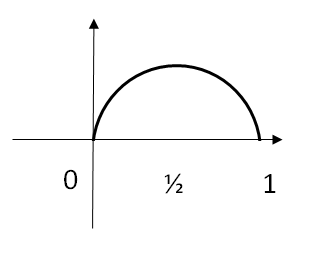
\includegraphics[width=2in]{Figure3.png}
  % \includegraphics[width=2in]{name.pdf} % uncomment this line and put the figure in the same folder as this document.
   \caption{Entropy graph}
   \label{fig:Figure3}
\end{figure}

Difference/Similarity between probability distributions.\\

KL Divergence\\

KL(p$||$q)$\triangleq\sum_{k=1}^KP_k\log\frac{P_k}{q_k}=\sum_kP_k\log{P_k}-\sum_kP_k\log{q_k}=-H(P)+H(P,q)$\\
H(P,q) is called the cross entropy.\\
\underline{Theorem 2.8.1} The Information Inequality\\
KL(P$||$q) $\geq$ 0\\
KL(P$||$q) = 0 $\Leftrightarrow$ P = q\\
The discrete distribution with maximum entropy is uniform distribution.\\
} %End of Large

\end{Section}
\begin{Section}{6}{Mutual Information}
\Large{
X, Y random variables\\
I(X;Y) = KL(P(X,Y) $||$ P(X)P(Y)) = $\sum_x\sum_yP(x,y)\log\frac{P(x,y)}{P(x)P(y)} \geq 0$\\
I(X;Y)=0 $\Leftrightarrow$P(x,y)=P(x)P(y) : independent\\
I(X;Y)=H(X)-H(X$|$Y) = H(Y) - H(Y$|$X) = $\sum_yP(y)H(X|Y=y)$\\
H(X$|$Y) is called the conditional entropy\\

PMI = Pointwise Mutual Information\\
PMI = $\log\frac{P(x,y)}{P(x)P(y)}=\log\frac{P(x|y)}{P(x)}=\log\frac{P(y|x)}{P(y)}$

For continuous, it is common to first discretize or quantize them by dividing the ranges of each variable into bins, and computing how many values fall in each histogram bin (Scott 1979)\\

MIC = Maximal Information Coefficient\\
m(X,Y) = $\frac{max_G I(X(G);Y(G))}{\log{min(X,Y)}}$\\
\itab{MIC=}\tab{max(X,Y)}\\
\itab{}\tab{x,y:xy<B}\\
B is the bound on the number of bins.\\
 

} %End of Large
\end{Section}

\end{document}

